% !TEX root = ../../thesis.tex

\newpage
\section{Rapid morphological exploration} % (fold)
\label{sec:morphology-variable}

In the previous section we showed how Poppy can be used to explore the actual role of morphology for humanoid behaviours. However, Poppy is a prototyping platform designed to test and experiment quickly several technological solution, especially thanks to modular properties, but until now, we did not actually evaluate it.

Therefore while we were working on a new design for Poppy's feet and exploring a design similar to "foot 1" (see \figurename~\ref{fig:pic_foot_1}), we decided to use this as a context to conduct an experiment into multiple variations of the foot morphology as an illustration of the methodology we have initiated with Poppy and presented in chapter~\ref{cha:methodology-review}.


The aim of this experiment is to quickly explore the effect of foot morphology on stability. Here, we are particularly interested in the stability of the head after a stepping impact. These impacts are quite challenging to simulate realistically and the natural compliance of the Poppy platform means it is even more important to test this on the real robot.

For the sake of lightness, the initial design of Poppy's feet only had one degree of freedom (DoF): pitch rotation. This configuration carried the inconvenience of preventing a proper parallel foot/ground contact. Thus, we developed several different feet with two degrees of freedom. Along with a standard motorized 2 DoF flat foot design, we also wanted to explore passive joints with springs. The use of passive joints allows for both lightness and reactive torque for stability.


\begin{figure}[p]
\centering
    \subfloat[][Foot\_1]{\label{fig:pic_foot_1}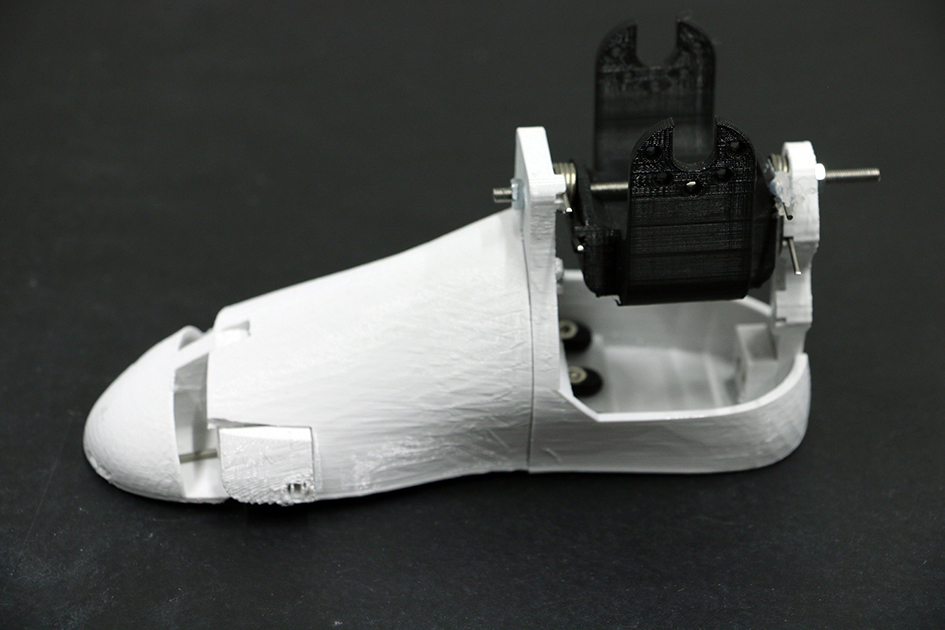
\includegraphics[width=0.45\linewidth]{pic_foot_1.JPG}}
    \hfil
    \subfloat[][Foot\_2]{\label{fig:pic_foot_2}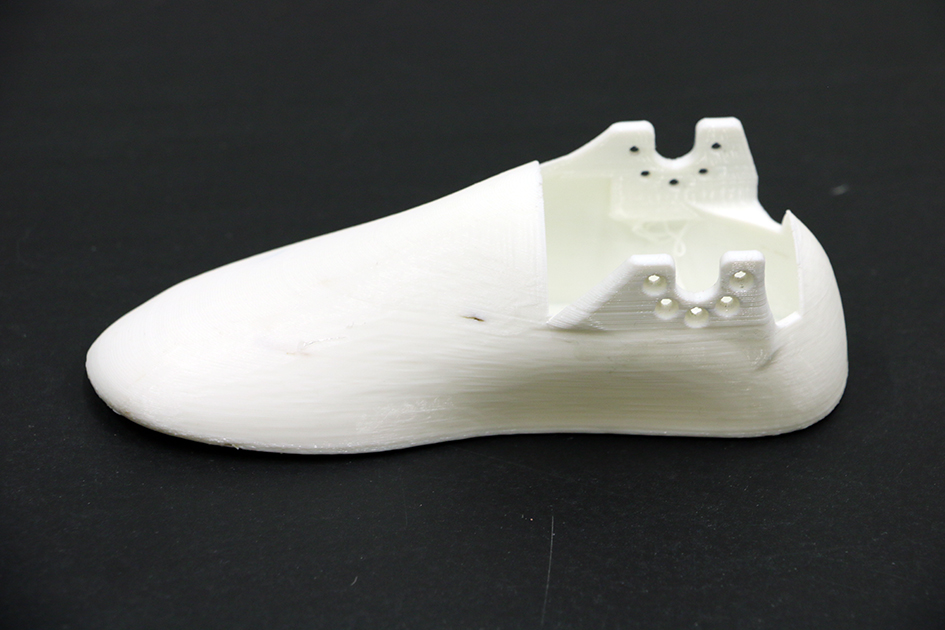
\includegraphics[width=0.45\linewidth]{pic_foot_2.JPG}}\\
    \subfloat[][Foot\_3]{\label{fig:pic_foot_3}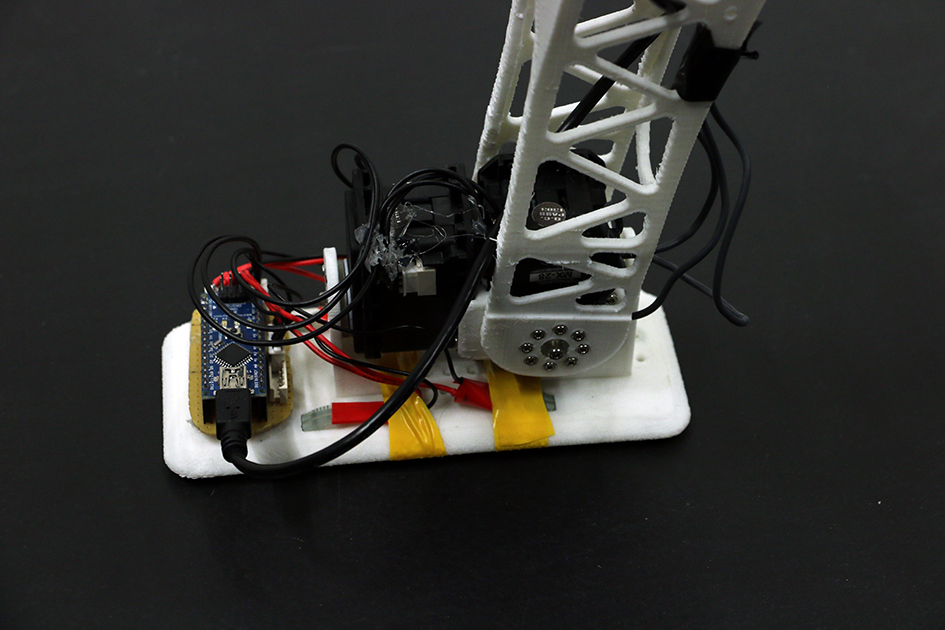
\includegraphics[width=0.45\linewidth]{pic_foot_3.JPG}}
    \hfil
    \subfloat[][Foot\_4]{\label{fig:pic_foot_4}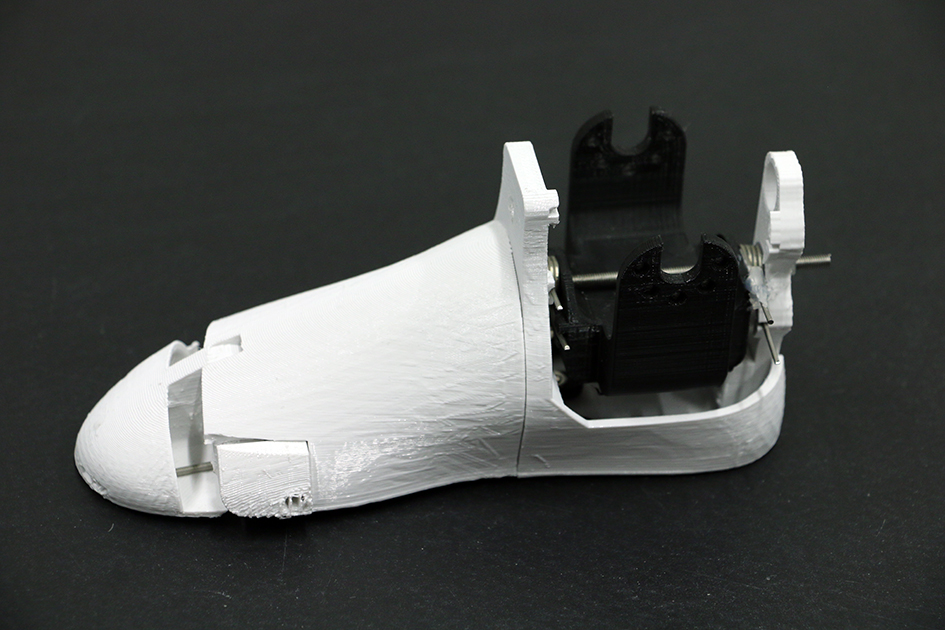
\includegraphics[width=0.45\linewidth]{pic_foot_4.JPG}}


    \subfloat[][Blueprints of the various foot designs studied in this experiments.]{\label{fig:foot_experience_blueprint}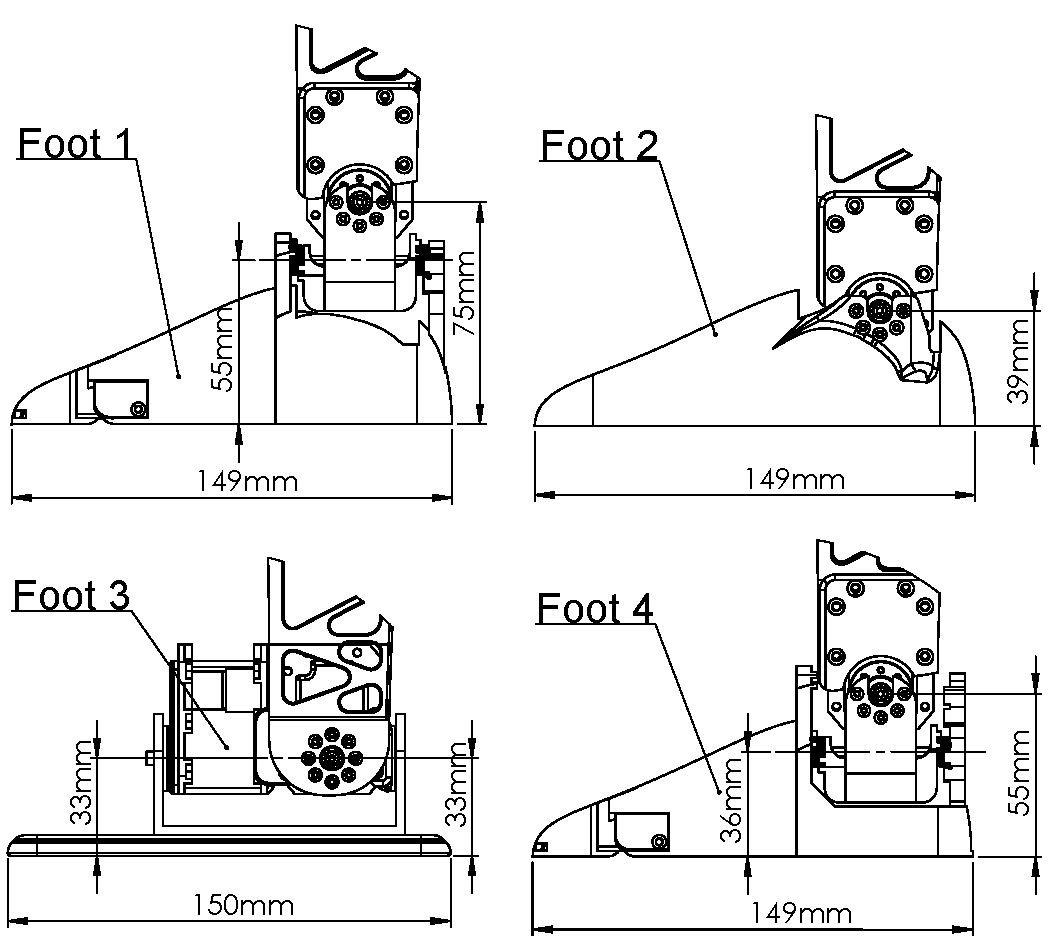
\includegraphics[width=0.95\linewidth]{foot_experience.pdf}}
    % \subfloat[][]{\label{fig:pic_shoe}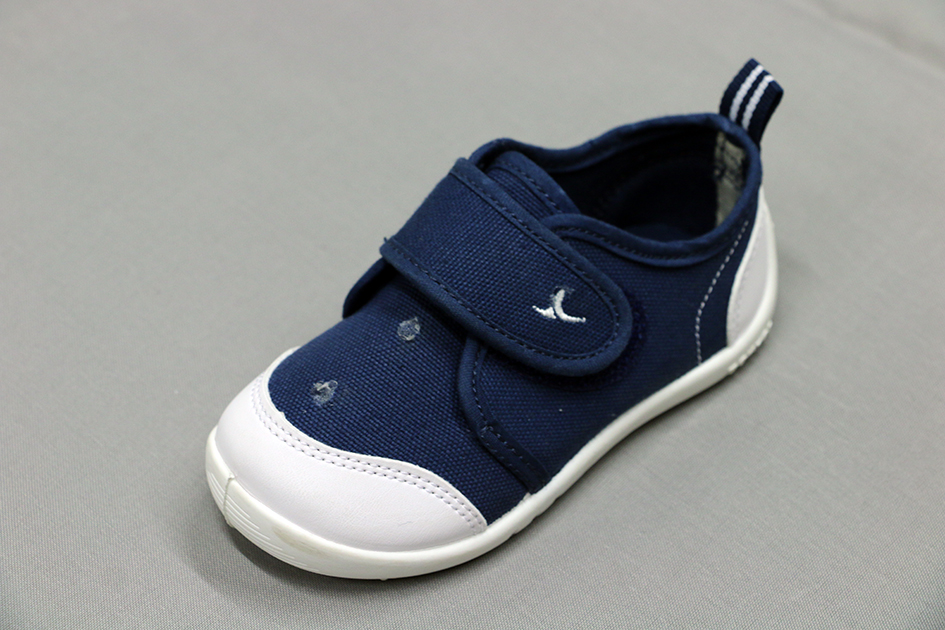
\includegraphics[width=0.48\linewidth]{pic_shoe.JPG}}
    \caption{Visual and technical descriptions of the foot designs explored in this experiments.}
    \label{fig:foot_variants}
\end{figure}


\begin{table}
    \begin{center}
        \begin{tabular}{ l c c c c }
        \hline
        \textbf{Type} & \textbf{Foot 1} & \textbf{Foot 2} & \textbf{Foot 3} & \textbf{Foot 4}\\
        \textbf{Double rotation} & Passive & No & Active & Passive\\
        \textbf{Human-like foot} & Yes & Yes & No & Yes\\
        \textbf{Toes} & Yes & No & No & Yes\\
        \textbf{Rotation axis height} & 75.70 mm & 33 mm & 39 mm & 35.5 mm\\
        \hline

        \end{tabular}
        \caption{Table summarizing the different types of feet used.\\
        \textbf{Passive double-rotation:}  one active rotation (motor: Dynamixel MX 28) for the sagittal plan and a passive rotation for the frontal plan with two springs.\\
        \textbf{Active double-rotation:}  A two motorized rotations (sagittal plan and frontal plan). No double-rotation:  one motorized rotation (sagittal plan).\\
        \textbf{Human-like foot:} a foot design resembling a human foot of a two year-old child (size: 130.7 mm shoes size: 23 EU). The feet were tested with and without shoes.\\
        \textbf{Rotation axis height:} the height between the axis of rotation of the sagittal plan and the floor without shoes.\\
        \textbf{Toes:} Indicates that the foot has toes.
        }
        \label{tab:table_feet}
    \end{center}
\end{table}


Moreover, it appeared that a proper foot/ground contact with convenient friction was difficult to obtain based only on 3D-printed material. One simple solution to this problem is to use a shoe which can provide a high friction and adapt slightly to imperfections on the ground. Furthermore, this solution also allows keeping the feet close to humans ones. Thus, the feet tested (with the exception of the flat foot) were designed from a moulding of the interior of a shoe. It is to be noted that we also included passive toes (with springs) on some of the feet tested for future work on locomotion. These toes should not have any significant impact on the criterion tested.


\subsection{Experimental setup} % (fold)
\label{sub:experimental_setup}

For this experiment, the robot simply stands upright secured by a slack strap on a fixed gantry. Different markers on the robot are tracked by a motion capture system at 100Hz (Natural Point OptiTrack). See figure \ref{fig:setup} for more details.

\begin{figure}[ht]
    \begin{center}
        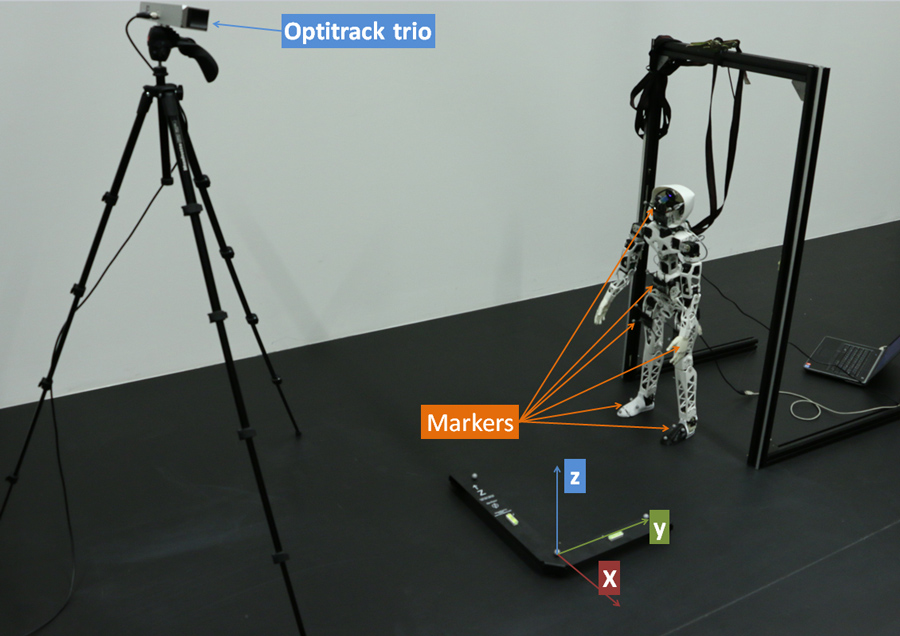
\includegraphics[width=0.9\linewidth]{pic_setup.jpg}
    \end{center}
    \caption{Experimental setup. The robot is secured by slack strap on a gantry and tracked by an OptiTrack trio device. Markers are placed on the feet, hips, abdomen, and on the head}
    \label{fig:setup}
\end{figure}

Four different feet were tested (cf. Table~\ref{tab:table_feet}). Three out of the four feet were tested both with and without shoes.


\subsection{Experiments} % (fold)

The feet were tested with a very simple discrete movement (see \codename~\ref{code:foot_mouvement}), representative of the kind of impacts that occur during walking. The robot performs a single step leftward with the left leg. The left foot is lifted (3cm) and then put back on the ground with a slight lateral displacement towards the exterior (5° at the level of the hip). The duration  of the whole movement is about 0.4 s and repeated 20 times for each configuration.

\lstinputlisting[
    language = Python,
    caption = {Discrete mouvement executed on Poppy},
    label = {code:foot_mouvement},
    float = p]
    {code/foot_mouvement.py}


\subsection{Results} % (fold)

Figures \ref{fig:head_x}, \ref{fig:head_y} and \ref{fig:head_z} respectively show the evolution of the position of the head marker in the $x$, $y$ and $z$ axis for each foot tested. Dotted vertical lines indicate the beginning and the end of the leg movement.

These figures show that the dynamics of the robot are not trivial, even for the simple movement we tested, the standard deviation is not negligible and shows how chaotic the reaction of such an impact can be. This particularity is another proof of the significance of the use of experimentation versus simulation.

We can clearly see that foot 3 (standard flat foot) behaves quite differently than the other feet tested. In particular in the $x$ and $y$ directions, we see that with this foot the head tends to move more towards the exterior (left of the robot) and towards the rear.
%% These differences may be explained by the larger ground contact surface
%% provided by the flat feet.

Regarding the effect of the shoes, results are less clear but most of the time (except for foot 1) differences occur between a given foot with and without shoes. The friction with the ground can explain these differences. Bare feet tend to slip more than those with shoes.


\begin{figure}[ht]
    \begin{center}
        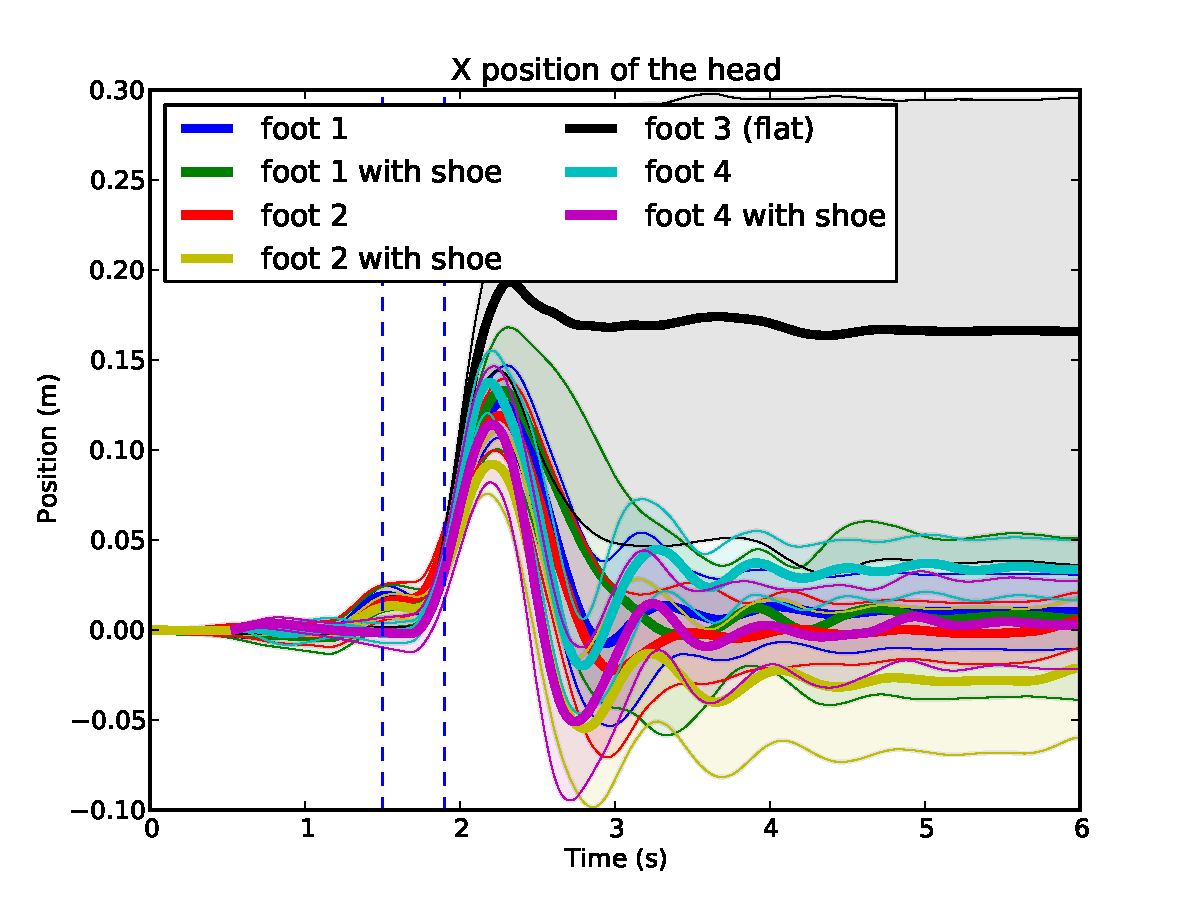
\includegraphics[width=\linewidth]{head_x.pdf}
    \end{center}
    \caption{Evolution of the position of the head in the $x$ axis for
    each foot tested (see \figurename~\ref{fig:foot_variants} for illustration of each foot)}
    \label{fig:head_x}
\end{figure}

\begin{figure}[ht]
    \begin{center}
        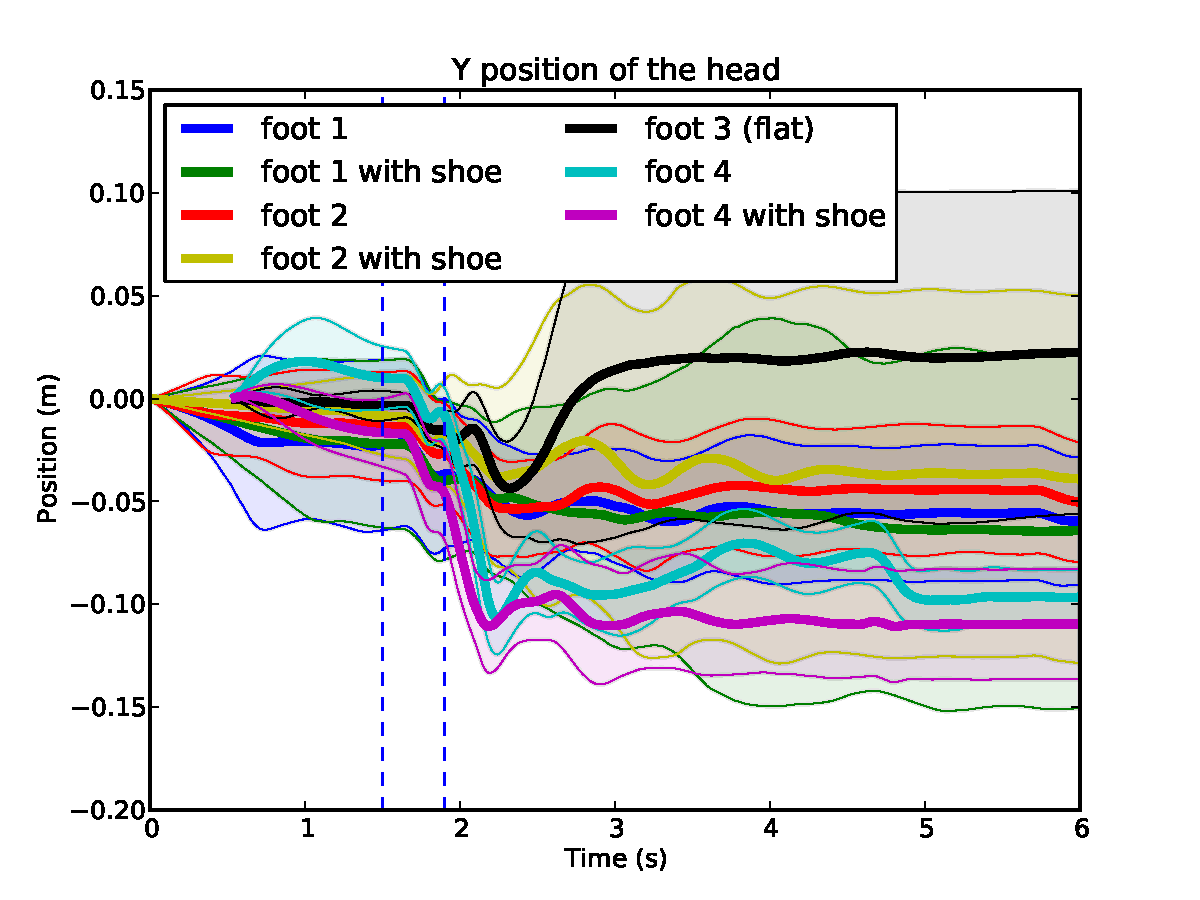
\includegraphics[width=0.95\linewidth]{head_y.pdf}
    \end{center}
    \caption{Evolution of the position of the head in the $y$ axis for
    each foot tested (see \figurename~\ref{fig:foot_variants} for illustration of each foot).}
    \label{fig:head_y}
\end{figure}

\begin{figure}[ht]
    \begin{center}
        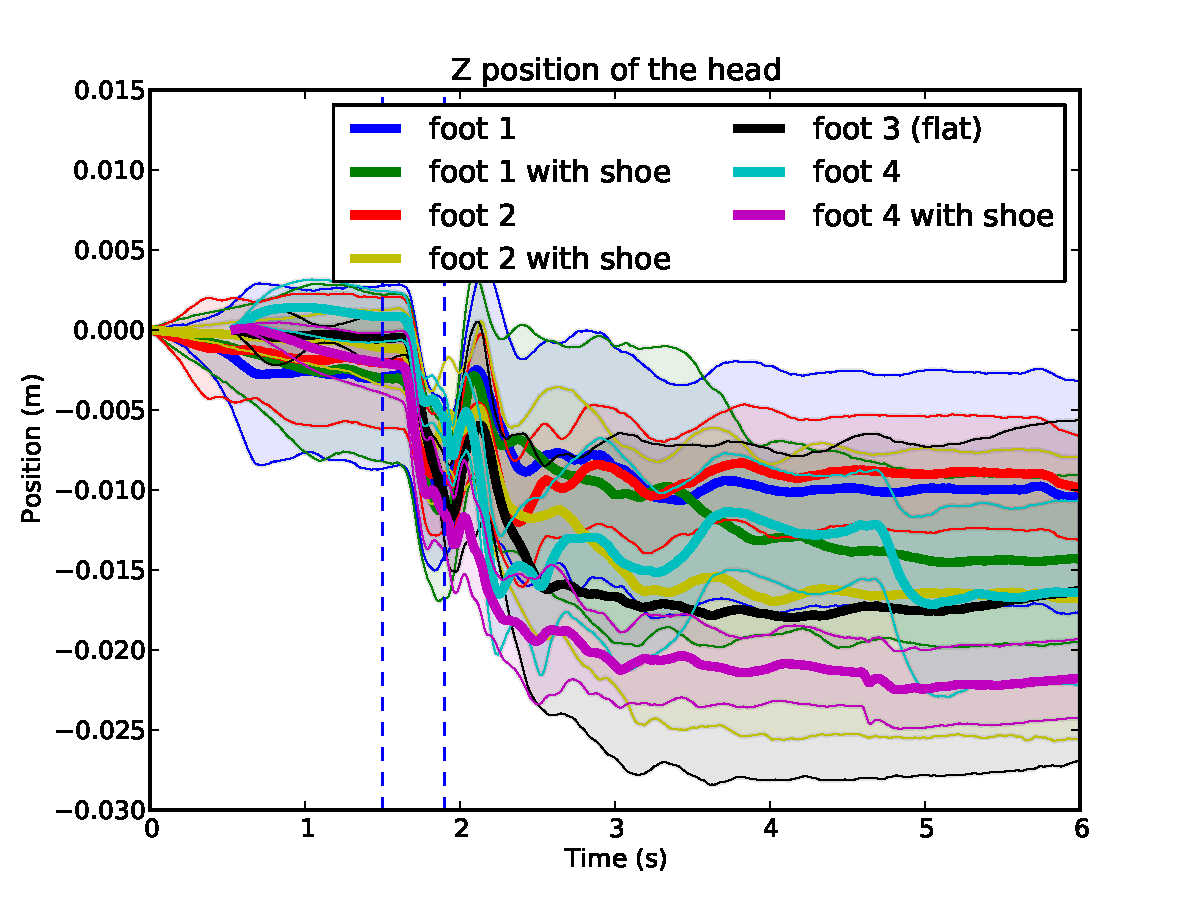
\includegraphics[width=0.95\linewidth]{head_z.pdf}
    \end{center}
    \caption{Evolution of the position of the head in the $z$ axis for
    each foot tested (see \figurename~\ref{fig:foot_variants} for illustration of each foot).}
    \label{fig:head_z}
\end{figure}


This first experiment allowed us to determine that the use of an active double rotation of the ankle may not be mandatory. Indeed, the behaviors observed with the passive feet were even better than with the flat feet with active rotation. Although a clear interpretation of this phenomenon is still difficult to propose, some hypotheses related to the weight (with one more motor feet are heavier) and the area of surface in contact with the ground (flat foot surface is bigger) have to be investigated.

Moreover, we observed that the shoes added extra friction in relation to the ground without really impairing the stability. Although rarely used in humanoid robotics, these early results encourage us to explore this possibility in more depth.

Finally the most important aspect for us was to actually evaluate the amount of time needed to conduct such experiments with Poppy. The starting point was "foot 1" as it was the work in progress. Thus morphological design modifications only concern foot 3 and 4:
\begin{itemize}
    \item \textbf{Foot 3 (flat):} Modifying Poppy’s initial foot design to permit the integration of two Dynamixel motors and the associated flat feet required 16 hours of CAD design. The printing of the whole required part (2 legs, 2 feet and 2 ankles) took approximately 30 hours on a low-cost FDM printer (Makerbot Replicator 2).
    \item \textbf{Foot 4:} While the difference with foot 1 concerns only one parameter (i.e. the joint position), the modification needed to produce foot 4 based on foot 1 was done in approximately 2 hours of CAD. Then the printing of the new part was achieved in 10 hours.
\end{itemize}

Then, conducting the whole experiment (i.e. design the leg motion, establishment of the experimental setup and data acquisition) was achieved in about one week with two people. \textbf{In particular, the actual experimentation involving changing Poppy's feet seven times and acquiring at least 20 trials for each took less than two days.}

\subsection{Reuse of this experiment} % (fold)

Everything necessary to obtain and use Poppy is available on our GitHub project page: \url{www.github.com/poppy_project}. Also, to complete the illustration of this Poppy use-case, we diffuse along with the present paper:
\begin{itemize}
     \item the whole setup materials i.e. the code used for the experiment and the 3D files to reproduce/modify each foot,
     \item the raw data acquired that include for each trial: all markers position, head IMU measurement and the complete motors data (proprioceptive position evaluation overtime),
     \item the code used to extract and plot the results presented.
\end{itemize}

All these materials are available on the repository associated with this experiment: \url{https://github.com/matthieu-lapeyre/Humanoids2014} and can be freely used e.g. for further investigation with the acquired data, or to reproduce and extend the experiment.

